\clearpage
\section{PARTIAL DERIVATIVES}
We begin the attack on the problem of finding derivatives
"one variable at a time." If $f: \F{R}^n\to \F{R}$ and $a\in \F{R}^n$, 
the limit
\begin{align}
    \lim_{h\to 0} \frac{f(a^1, \cdots, a^i+h, \cdots, a^n) - f(a^1, \cdots, a^n)}{h}
\end{align}

If it exists, is denoted $\R{D}_if(a)$, and called the $i$th \textbf{partial derivative}\index{Derivative!partial} 
of $f$ at $a$. It is important to note that $\R{D}_if(a)$ is the ordinary derivative of
a certain fucntion; in fact, if $g(x) = f(a^1, \cdots, x, \cdots, a^n)$, then $\R{D}_if(a) = g'(a^i)$.
This means that $\R{D}_if(a)$ is the slope of the tangent line at $(a, f(a))$ to the 
curve obtained by intersecting the tangent line of $f$ with the plane $x^j=a^j, j\neq i$ \figref{Fig 2-1}.
It also means that computation of $\R{D}_if(a)$ is a problem we can already solve. If $f(x^1, \cdots, x^n)$
is given by some formula involving $x^1, \cdots, x^n$, then we find $\R{D}_if(a)(x^1, \cdots, x^n)$ by differentiating 
the function whose value at $x^i$ is given by the formula when all $x^j$, for $j\neq i$, are 
thought of as constants. For example, if $f(x, y) = 2xy\cos(xy^2)$. If, instead, $f(x, y)= x^y$, then 
$\R{D}_1f(x, y) = yx^{y-1}$ and $\R{D}_2f(x, y) = x^y \ln x$. 

\begin{figure}[!htb]
    \centering
    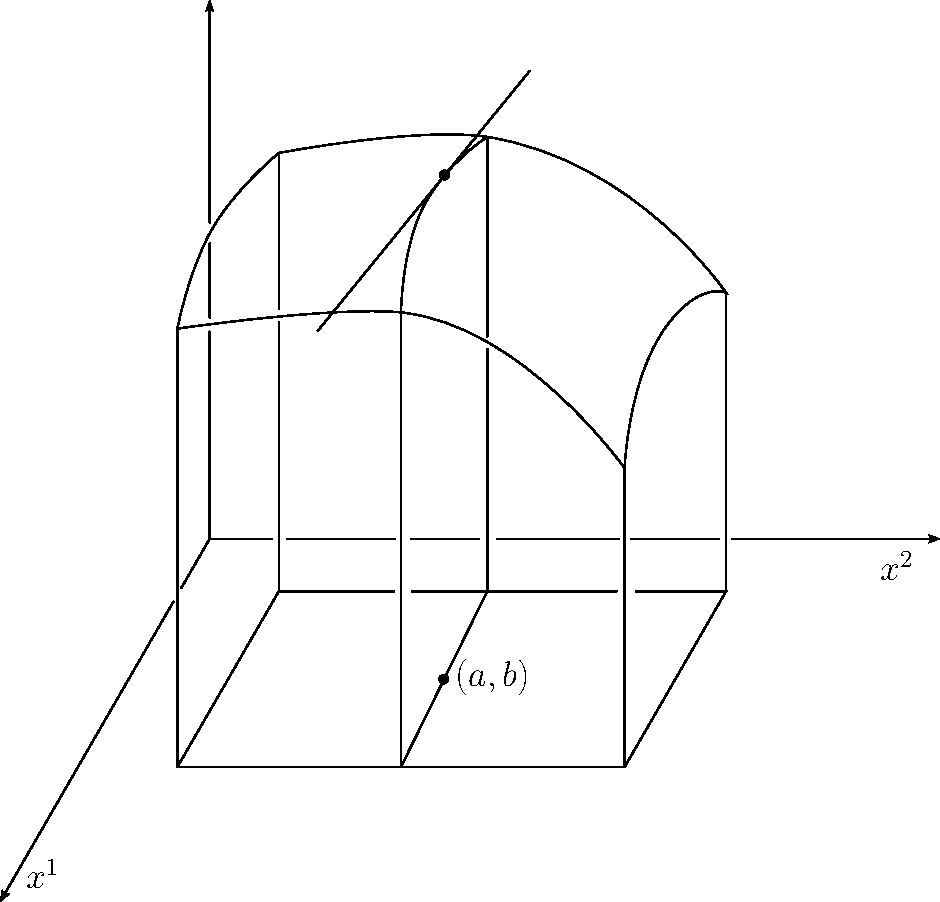
\includegraphics[width=.75\linewidth]{./pics/Fig2-1.pdf}
    \caption{}
    \label{Fig 2-1}
\end{figure}

With a littw practice (e.g., the problems at the end of this
section) you should acquire as great a facility for computing
$\R{D}_if$ as you already have for computing ordinary derivatives.

If $\R{D}_if(x)$ exists for all $x\in \F{R}^n$, we obtain a fucntion at $x$, that 
is, $\R{D}_j(\R{D}_if)(x)$, is often denoted $\R{D}_{i,j}f(x)$. Note that this notation 
reverses the order of $i$ and $j$. As a matter of fact, the
order is usually irrelevant, since most functions (an exception is
given in the problems) satisfy $\R{D}_{i,j}f = \R{D}_{j,i}f$· There are various
delicate theorems ensuring this equality; the following theorem
is quite adequate. We state it here but postpone the proof until later (Problem 3-28).

\begin{theorem}
    If $\R{D}_{i,j}f$ and $\R{D}_{j,i}f$ are continuous in an open set containing $a$, then 
    \begin{align}
        \R{D}_{i,j}f(a) = \R{D}_{j,i}f(a)
    \end{align}
\end{theorem}

The function $\R{D}_{i,j}f$ is called a \textbf{second-order (mixed) partial derivative}\index{Partial derivative!second-order (mixed)}\index{Derivative!partial!second-order (mixed)}
of $f$.Higher-order (mixed) partial derivatives are defined in the obvious way.
Clearly Theorem 2-5 can be used to prove the equality of higher-order mixed
partial derivatives\index{Partial derivative!higher-order (mixed)}\index{Derivative!partial!higher-order (mixed)} under appropriate conditions.
The order of $i_1, \cdots ,i_k$ is completely immaterial in $\R{D}_{i_1,\cdots,i_k}f$
if $f$ has continuous partial derivatives of all orders. A function
with this property is called a $C^\infty$ function\index{$C^\infty$}\index{Function!$C^\infty$}. In later chapters
it will frequently be convenient to restrict our attention to $C^\infty$
functions.

Partial derivatives will be used in the next section to find
derivatives. They also have another important use-finding
maxima\index{Maxima|(} and minima\index{Minima|(} of functions.

\begin{theorem}
  Let $A\subset \F{R}^n$. If the maximum (or minimum) of $f:A\to \F{R}^n$ occurs at a 
  point $a$ in the interior of $A$ and $\R{D}_if(a)$ exists, then $\R{D}_if(a) = 0$.
\end{theorem}

\begin{proof}
  Let $g_i(x) = f(a^1, \cdots, x, \cdots, a^n)$. Clearly $g_i$ has a maximum (or minimum)
  at $a^i$, and $g_i$ is defined in an open interval containing 
  $a^i$. Hence $0 = g_i(a^i) = \R{D}_if(a)$.
\end{proof}

The reader is reminded that the converse of Theorem 2-6
is false even if $n=1$ (if $f:\F{R}\to \F{R}$ is defined by $f(x) = x^3$, then $f'(0) = 0$, but 
0 is not even a local maximum or minimum). If $n>1$, the converse of Theorem 2-6 may fail 
to be true in a rather spectacular way. Suppose, for example, that $f:\F{R}^2\to \F{R}$ is defined 
$f(x, y) = x^2-y^2$ (\figref{Fig 2-2}). Then $\R{D}_1f(0, 0) = 0$ because $g_1$ 
has a minimum at 0, while $\R{D}_2f(0) = 0$ because $g_2$ has a maximum at 0. 
Clearly $(0, 0)$ is neither a reletive maximum nor reletive minimum.

\begin{figure}[!htb]
    \centering
    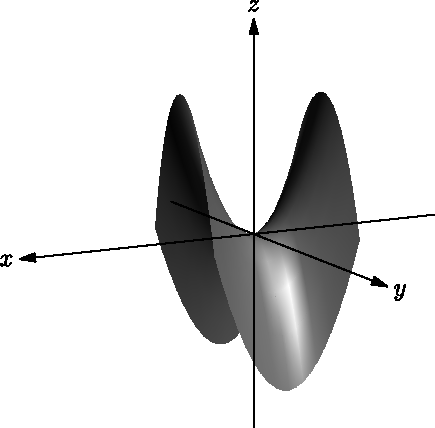
\includegraphics[width=.75\linewidth]{./pics/Fig2-2.pdf}
    \caption{}
    \label{Fig 2-2}
\end{figure}

If Theorem 2-6 is used to find the maximum or minimum of
$f$ on $A$, the values off at boundary points must be examined
separately-a formidable task, since the boundary of $A$ may
be all of $A$! Problem 2-27 indicates one way of doing this,
and Problem 5-16 states a superior method which can often
be used.
\index{Maxima|)}
\index{Minima|)}

\begin{problems}
    \problem{Find the partial derivatives of the following functions:\vspace*{-1em}
        \begin{multicols}{2}
        \begin{enumerate}[label={\upshape(\alph*)}]
            \item $f(x,y,z)=x^{y}$
            \item $f(x,y,z)=z$
            \item $f(x,y)=\sin(x\sin y)$
            \item $f(x,y,z)=\sin(x\sin(y\sin z)$ 
            \item $f(x,y,z)=x^{y^{z}}$
            \item $f(x,y,z)=x^{y+z}$
            \item $f(x,y,z)=(x+y)^{z}$
            \item $f(x,y)=\sin{(xy)}$
            \item $f(x,y)=[\sin{(xy)}]^{\cos{3}}$
        \end{enumerate}\end{multicols}
        }
    \problem{Find the partial derivatives of the following functions (where $g:\F{R}\to \F{R}$ is continuous):\vspace*{-1em}
        \begin{multicols}{2}
        \begin{enumerate}[label={\upshape(\alph*)}]
            \item $\displaystyle f(x, y) = \int_{a}^{x+y}{g}$
            \item $\displaystyle f(x, y) = \int_{y }^{x }{g }$
            \item $\displaystyle f(x, y) = \int_{a }^{xy }{g }$
            \item $\displaystyle f(x, y) = \int_{a }^{\left(\int_{b }^{y }{g }\right)}{g }$
        \end{enumerate}\end{multicols}
        }
    \problem{If $f(x, y)$ defined as follows:
            \begin{align*}
                f(x, y) = x^{x^{x^{x^y}}} + (\ln x)\cdot 
                    \left(\arctan \left(\arctan\left(\sin \left(\cos xy  - \ln (x+y) \right)\right)\right)\right)
            \end{align*}
            find $\R{D}_2f(1, y)$. \textit{Hint:} There is an easy way to do this.
        } 
    \problem{Find the partial derivatives off in terms of the derivatives of $g$ and
        $h$ if \vspace*{-1em}
        \begin{multicols}{2}
        \begin{enumerate}[label={\upshape(\alph*)}]
            \item $f(x,y) =g(x)h(y)$
            \item $f(x,y) =g(x)^{h{(y)}}$
            \item $f(x,y) =g(x)$
            \item $f(x,y) =g(y)$
            \item $f(x,y) =g(x+y)$
        \end{enumerate}\end{multicols}
        }
    \problem[*]{Let $g_1,g_2:\F{R}^2\to \F{R}$ be conttinuous. Define $f:\F{R}^2\to \F{R}$ by 
            \begin{align*}
                f(x, y) = \int_{0}^{x }{g_1(t, 0)  \mathrm{d}t} + \int_{0}^{y}{g_2(x, t) \mathrm{d}t}
            \end{align*}
            \begin{enumerate}[label={\upshape(\alph*)}]
                \item Show that $\R{D}_2f(x, y) = g_2(x, y)$.
                \item How should $f$ be defined so that $\R{D}_1f(x, y) = g_1(x, y)$?
                \item Find a function $f:\F{R}^2\to \F{R}$ such that $\R{D}_1f(x, y) = x$ and 
                    $\R{D}_2f(x, y)$ $=y$. Find one such that $\R{D}_1f(x, y) = y$ and $\R{D}_2f(x, y) = x$.
            \end{enumerate}
        }
    \problem[*]{If $f:\F{R}^2\to \F{R}$ and $\R{D}_2f = 0$, show that $f$ is independent of the second variable.
        If $\R{D}_1f = \R{D}_2f = 0$, show that $f$ is constant.}
    \problem[*]{Let $A = \{(x, y)\in \F{R}^2: x<0,\text{ or } x\ge 0\text{ and } y\neq 0\}$.
            \begin{enumerate}[label={\upshape(\alph*)}]
                \item If $f:A\to \F{R}$ and $\R{D}_af = \R{D}_2f = 0$, show that $f$ is constant 
                    \textit{Hint:} Note that any two points in $A$ can be connected by a sequence 
                    of lines each parallel to one of the axes.
                \item Find a fucntion $f:A\to \F{R}$ such that $\R{D}_2f = 0$ but $f$ is not independent
                    of the second variable. 
            \end{enumerate}
        } 
    \problem{Define $f:\F{R}^2\to \F{R}$ by 
            \begin{align*}
                f(x, y) = \left\{\begin{aligned}
                    & xy \cdot \frac{x^2 -y^2}{x^2 + y^2} && (x, y) \neq 0 \\
                    & 0 && (x, y) = 0
                \end{aligned}\right.
            \end{align*}
            \begin{enumerate}[label={\upshape(\alph*)}]
                \item Show that $\R{D}_2f(x, 0) = x$ for all $x$ and $\R{D}_1f(0, y)= -y$ for all $y$.
                \item Show that $\R{D}_{1, 2}f(0, 0) \neq \R{D}_{2, 1}f(0, 0)$.
            \end{enumerate}
        }
    \problem[*]{ Define $f:\F{R}\to \F{R}$ by 
            \begin{align*}
                f(x, y) = \left\{\begin{aligned}
                    & \mathrm{e}^{-x^{-2}} && x \neq 0 \\
                    & 0 && x = 0
                \end{aligned}\right.
            \end{align*}
        Show that $f$ is a $C^\infty$ fucntion, and $f^{(i)}(0) = 0$ for all $i$. 
        \textit{Hint:} The limit $f'(0) = \lim_{h\to 0}{\frac{\mathrm{e}^{-h^{-2}}}{h}} 
            = \lim_{h\to 0}{\frac{1/h}{\mathrm{e}^{h^{-2}}}}$ can be evaluated by L'Hospital's 
            rule. It is easy enough to find $f'(x)$ for $x\neq 0$, and $f''(0)=\displaystyle\lim_{h\to 0}{f'(h)/h}$
            can be then be found by L'Hopital's rule
        }
    \problem[*]{Let 
            \begin{align*}
                f(x) = \left\{\begin{aligned}
                    & \mathrm{e}^{-(x-1)^{-1}} \cdot \mathrm{e}^{-(x+1)^{-2}} && x\in (-1, 1) \\
                    & 0 && x\notin (-1, 1)
                \end{aligned}\right.
            \end{align*}
            \begin{enumerate}[label={\upshape(\alph*)}]
                \item Show  that $f:\F{R}\to \F{R}^2$ is a $C^\infty$ function which is positive 
                    on $(-1, 1)$ and 0 else 0 elsewhere.
                \item Show that there is a $C^\infty$ fucntion $g:\F{R}\to [0, 1]$ such that $g(x) = 0$ for $x<0$ and 
                    $g(x) = 1$ for $x\ge \varepsilon$. \textit{Hint:} If $f$ is a $C^\infty$ function which is positive
                    on $(0, \varepsilon)$ and 0 elsewhere, let $g(x) = \int_{0}^{x }{{f}\big/{\int_{0 }^{\varepsilon }{f }}}$.
                \item If $a\in \F{R}^n$, define $g:\F{R}^n\to \F{R}$ by 
                    \begin{align*}
                        g(x) = f\left(\left[x^1,-a^1\right]/\varepsilon\cdot \cdots \cdot f\left[x^n - a^n\right]/\varepsilon\right)
                    \end{align*} 
                    Show that $g$ is a $C^\infty$ function which is positive on 
                    \begin{align*}
                        \left(a^1-\varepsilon, a^1+\varepsilon\right) \times \cdots, \times\left(a^n-\varepsilon, a^n+\varepsilon\right)
                    \end{align*}
                    and zero elsewhere
                \item If $A\subset \F{R}^n$ is open and $C\subset A$ is compact, show that there is a 
                    non-negative $C^\infty$ function $f:A\to \F{R}$ such that $f(x)>0$ for $x\in C$ anf $f(x) = 0$
                    outside of some closed set contained in $A$.
                \item Show that we can choose such an $f$ so that $f:A\to [0, 1]$ and $f(x) = 1$ for $x\in C$. 
                    \textit{Hint:} If the function $f$ of (d) satisfies $f(x)\ge \varepsilon$ for $x\in C$, consider 
                    $g\circ f$, where $g$ is the function of (b).
            \end{enumerate}
        }
    \problem{Define $g, h:\{x\in \F{R}^2: |x|\le 1\} \to \F{R}^2$ by 
            \begin{align*}
                & g(x, y) = \left(x, y, \sqrt{1-x^2-y^2}\right) \\
                & h(x, y) = \left(x, y, -\sqrt{1-x^2-y^2}\right) 
            \end{align*}
            Show that the maximum of $f$ on $\{x\in \F{R}^2:|x|=1\}$ is either the 
            maximum of $f\circ g$ or the maximum of $f\circ h$ on $\{x\in \F{R}^2:|x|\le 1\}$.
        }
\end{problems}